\documentclass[12pt, a4paper, titlepage,twoside]{article}

\usepackage{ngerman}
\usepackage{lmodern}
\usepackage{amssymb }
\usepackage{subfig}
\usepackage{colortbl}

\title{Primfaktorzerlegung und Primzahltests}
\author{Maximilian Scholz  \\
	Technische Universit\"at Hamburg-Harburg \\
}

\date{\today}
\begin{document}
	\maketitle
	%this file is prim_abstract.tex
	\begin{abstract}
		\label{sec:abstract}
		
		Mit dieser Ausarbeitung im Rahmen des Proseminars Mathematik will ich eine Einleitung in die Welt der Primzahlen im Allgemeinen und der Primfaktorzerlegung im besonderen schaffen. \\
		Ich beginne mit einer Einleitung zu den Primzahlen und zeige anhand von Beispielen, wie sich die Problematik der Primfaktorzerlegung auf verschiedene Wege angehen l\"asst. Hierzu beleuchte ich nicht nur die Algorithmen im einzelnen sondern zeige auch, welche Werkzeuge benutzt werden und erkl\"are auch diese detaillierter, da mir diese Herleitungen in der Fachliteratur oft zu kurz kommen.\\
		Letztendlich ist mein Ziel Verst\"andnis in einem sehr begrenzten Bereich zu schaffen anstatt in die Breite zu gehen, denn nur durch wirkliches Verst\"andnis k\"onnen neue Entdeckungen wie der zum Beispiel der AKS-Algorithmus gemacht werden.
	\end{abstract}
	\tableofcontents % Um ein Inhaltsverzeichnis zu generieren 
	\newpage	
	 % this file is prim_primzahlen.tex	
	
	\section{Einf\"uhrung in Primzahlen} 
	\label{sec:primzahlen}
	Die wichtigsten Dinge die es zu Primzahlen im Bezug auf diesen Text gibt lassen sich wie folgt zusammenfassen:

	\begin{itemize}
		\item Definition: Jede nat\"urliche Zahl $>1$, die nur von sich selber und  $1$ geteilt wird, ist eine Primzahl. Dies l\"asst sich auch so beschreiben, dass eine Primzahl nur beim Teilen durch $1$ und sich selber keinen Rest hat.
		\item Der griechische Mathematiker Euklid hat bewiesen, dass es unendlich Primzahlen gibt. W\"urde dies nicht gelten, k\"onnte es zu Problemen bei modernen Kryptographischen Verfahren kommen, da diese auf immer gr\"oßer werdenden Primzahlen beruhen. 
		\item  Ebenfalls von Euklid kommt der Beweis daf\"ur, dass sich jede nat\"urliche Zahl als Produkt von Primzahlen darstellen l\"asst, wobei man hierf\"ur die triviale Multiplikation mit der $1$ hinzuf\"ugen muss. Sp\"ater fand Gauss heraus, dass diese sogenannte Zerlegung bis auf die Reihenfolge der einzelnen Elemente eindeutig ist. \\
		Dies ist besonders interessant weil es uns erm\"oglicht zusammengesetzte Zahlen $($also Zahlen, die nicht prim sind$)$ daran zu erkennen, dass wir einen Faktor ungleich der Zahl oder 1 gefunden haben. Außerdem birgt dies die Grundlage zu manchen Angriffen auf Kryptografische Verfahren wie RSA, auf die in diesem Text allerdings nicht weiter eingegangen werden.
	\end{itemize}
	
	Dieser Text wird sich im weiteren Verlauf vor allem mit der Zerlegung von Zahlen in deren Primfaktoren befassen. 
	%this file is prim_eratosthenes.tex


	\section{Sieb des Eratosthenes}
	 \label{sec:eratosthenes}
	Das Sieb des Eratosthenes ist ein etwa 2000 Jahre altes Verfahren, um alle Primzahlen in einem gegebenen Zahlenbereich zu finden. 
	\subsection{Funktionsweise}
	Das Sieb des Eratosthenes bestimmt alle Primzahlen N, indem es alle zusammengesetzten Zahlen streicht, daher der Name: Sieb.\\
	Das Abbruchkriterium ist ein sch\"önes Beispiel wie unn\"ötiger Aufwand vermieden werden kann.
	\subsection{Beispiel}
	Bevor die genaue Funktionsweise behandelt wird, hier einmal ein Beispiel f\"ür die Funktionsweise der Methode.\\
	\ \\
	\ \\
	\begin{table}[!ht] 
		\centering
		
		\begin{tabular}{|c|c|c|c|c|c|c|c|c|c|}
			\hline
			0  &  1 &  2 &  3 &  4 &  5 &  6 &  7 &  8 &  9 \\
			\hline
			10 & 11 & 12 & 13 & 14 & 15 & 16 & 17 & 18 & 19 \\
			\hline
			20 & 21 & 22 & 23 & 24 & 25 &  &  &  &  \\
			\hline
		\end{tabular}
		\caption{Eratosthenes 1}
		\label{tab:eratosthenes1}
	\end{table}
	
	Zu Beginn werden alle Zahlen im Bereich, in dem nach Primzahlen gesucht werden soll aufgeschrieben.
	
	\begin{table}[!ht] 
		\centering
		\begin{tabular}{|c|c|c|c|c|c|c|c|c|c|}
			\hline
			\cellcolor{red}0  &  \cellcolor{red}1 &  2 &  3 &  4 &  5 &  6 &  7 &  8 &  9 \\
			\hline
			10 & 11 & 12 & 13 & 14 & 15 & 16 & 17 & 18 & 19 \\
			\hline
			20 & 21 & 22 & 23 & 24 & 25 &  &  &  &  \\
			\hline
		\end{tabular}
		\caption{Eratosthenes 2}
		\label{tab:eratosthenes2}
	\end{table}
	
	Die Zahlen $0$ und $1$ sind per Definition keine Primzahlen, wir können sie somit streichen.	 	
	
	\begin{table}[!ht] 
		\centering
		\begin{tabular}{|c|c|c|c|c|c|c|c|c|c|}
			\hline
			\cellcolor{red}0  & \cellcolor{red} 1 &  2 &  3 &  \cellcolor{red}4 &  5 & \cellcolor{red} 6 &  7 & \cellcolor{red} 8 &  9 \\
			\hline
			\cellcolor{red}10 & 11 & \cellcolor{red}12 & 13 & \cellcolor{red}14 & 15 & \cellcolor{red}16 & 17 & \cellcolor{red}18 & 19 \\
			\hline
			\cellcolor{red}20 & 21 & \cellcolor{red}22 & 23 & \cellcolor{red}24 & 25 & \ & \ & \ & \ \\
			\hline
		\end{tabular}
		\caption{Eratosthenes 3}
		\label{tab:eratosthenes3}
	\end{table}
	
	Die erste nicht gestrichene Zahl ist $2$. Gleichzeitig ist $2$ die erste Primzahl. Da alles Zahlen die durch $2$ teilbar sind nicht prim sind, können wir alle geraden Zahlen streichen. 
	
	\begin{table}[!ht] 
		\centering
		\begin{tabular}{|c|c|c|c|c|c|c|c|c|c|}
			\hline	 		 			
			\cellcolor{red}0  & \cellcolor{red} 1 &  2 &  3 & \cellcolor{red}4 &  5 & \cellcolor{red} 6 &  7 & \cellcolor{red} 8 &  \cellcolor{red}9 \\
			\hline
			\cellcolor{red}10 & 11 & \cellcolor{red}12 & 13 & \cellcolor{red}14 & \cellcolor{red}15 & \cellcolor{red}16 & 17 & \cellcolor{red}18 & 19 \\
			\hline
			\cellcolor{red}20 & \cellcolor{red}21 & \cellcolor{red}22 & 23 & \cellcolor{red}24 & 25 &  &  &  &  \\
			\hline
		\end{tabular}
		\caption{Eratosthenes 4}
		\label{tab:eratosthenes4}
	\end{table}
	
	Die n\"achste nicht gestrichene Zahl ist $3$. Somit ist auch $3$ eine Primzahl. Wieder werden alle Vielfachen von $3$ gestrichen, da sie durch $3$ teilbar, und somit nicht prim, sind.
	
	\begin{table}[!ht] 
		\centering
		\begin{tabular}{|c|c|c|c|c|c|c|c|c|c|}
			\hline	 		 			
			\cellcolor{red}0  & \cellcolor{red} 1 &  2 &  3 & \cellcolor{red}4 &  5 & \cellcolor{red} 6 &  7 & \cellcolor{red} 8 &  \cellcolor{red}9 \\
			\hline
			\cellcolor{red}10 & 11 & \cellcolor{red}12 & 13 & \cellcolor{red}14 & \cellcolor{red}15 & \cellcolor{red}16 & 17 & \cellcolor{red}18 & 19 \\
			\hline
			\cellcolor{red}20 & \cellcolor{red}21 & \cellcolor{red}22 & 23 & \cellcolor{red}24 & \cellcolor{red}25 &  &  & &  \\
			\hline
		\end{tabular}
		\caption{Eratosthenes 5}
		\label{tab:eratosthenes5}
	\end{table}	
	
	Die $4$ ist schon gestrichen, da sie durch $2$ teilbar ist. Die n\"achste nicht gestrichene Zahl ist $5$. Damit ist $5$ die n\"achste Primzahl und alle Vielfachen von $5$ werden gestrichen.
	
	\begin{table}[!ht] 
		\centering
		\begin{tabular}{|c|c|c|c|c|c|c|c|c|c|}
			\hline	 		 			
			\cellcolor{red}0  & \cellcolor{red} 1 &  \cellcolor{green}2 &  \cellcolor{green}3 & \cellcolor{red}4 &  \cellcolor{green}5 & \cellcolor{red} 6 &  \cellcolor{green}7 & \cellcolor{red} 8 &  \cellcolor{red}9 \\
			\hline
			\cellcolor{red}10 & \cellcolor{green}11 & \cellcolor{red}12 & \cellcolor{green}13 & \cellcolor{red}14 & \cellcolor{red}15 & \cellcolor{red}16 & \cellcolor{green}17 & \cellcolor{red}18 & \cellcolor{green}19 \\
			\hline
			\cellcolor{red}20 & \cellcolor{red}21 & \cellcolor{red}22 & \cellcolor{green}23 & \cellcolor{red}24 & \cellcolor{red}25 &  &  &  &  \\
			\hline
		\end{tabular}
		\caption{Eratosthenes 6}
		\label{tab:eratosthenes6}			
	\end{table}
	
	Da nur die Zahlen bis $25$ betrachtet werden, ist die Methode an dieser Stelle fertig. Mit $5=\sqrt{25}$ haben wir den kleinsten Teiler von 25 gefunden und damit alle m\"oglichen Teiler der Zahlen $<25$. 
	
	\subsection{Mathematik}
	Die Methode des quadratischen Siebes l\"asst sich wie folgt beschreiben:
	\begin{itemize}
		
		\item W\"ahle eine nat\"uriche Zahl $n > 1$. Dies ist die obere Grenze der Zahlen, in denen nach Primzahlen gesucht wird.
		\item Die kleinste noch nicht gestrichene Zahl $m$ mit $2 \leq m$ wird die aktuelle Zahl.
		\item Wenn $m^2 \leq n$ ist, streiche alle Vielfachen $c\cdot m$ ($c \in \mathbb{N} $ ) mit $m^2 \leq cm \leq n$
		\item \"Ubrig bleiben alle Primzahlen zwischen $0$ und $n$. 
	\end{itemize}
	 % this file is prim_pollard.tex
	 % this file is prim_tools.tex
 
  
  \section{Pollard Rho Methode}
  \label{sec:pollard}
  \subsection{Geburtstagsproblem}
  Die Idee des Geburtstagsproblems ist die Frage, wie hoch die Wahrscheinlichkeit auf einem Geburtstag mit $N$ Personen ist, dass zwei am gleichen Tag Geburtstag haben.\\
  Eine M\"oglichkeit das Problem einfacher zu machen ist, stattdessen das inverse Problem zu betrachten, also wie hoch die Wahrscheinlichkeit $(P)$ ist, dass kein Geburtstag doppelt vorkommt.\\
  Bei einem Besucher ist die Wahrscheinlichkeit
  \[P(1)=\frac{356}{356}\] 
  da alle $356$ Tage zur Wahl stehen. Bei zwei Besuchern ist die Wahrscheinlichkeit 
  \[P(2)=\frac{356}{356}\cdot \frac{364}{365}\]
  bei drei Besuchern gilt  
  \[P(3)=\frac{356}{356}\cdot \frac{364}{365} \cdot \frac{363}{365}\]
  Im Allgemeinen gilt: 
  \[P(N)= \frac{365 \cdot 364 ... (365-N+1)}{365^N}\]
  Da wir gro\ss e Primzahlen betrachten werden interessiert uns auch das Verhalten des Geburtstagsproblems f\"ur gro\ss e $N$.
  Beim Betrachten von vielen Geburtstagen mit $N$ Personen, liegt, f\"ur gro\ss e N, die Zahl der Wiederholungen die man durchschnittlich braucht um einen doppelten Geburtstag zu erhalten bei: 
  \[\sqrt{\frac{\pi \cdot N}{2}}\]
  
  \subsection{Hase Igel Algorithmus}
  Der Hase Igel Algorithmus wird benutzt, um Zyklen in Folgen zu finden. Die Idee ist, die Folge mit zwei Zeigern zu durchlaufen, dem Hase und dem Igel, die auf dem gleichen Feld starten. Falls es einen Zyklus in der Folge gibt, werden sich Hase und Igel irgendwann wieder treffen, da der schnellere Hase den langsameren Igel einholt und \"uberrundet.
  \subsubsection{Beispiel}
  In diesem Beispiel ist eine Folge zu sehen, die einen Zyklus beinhaltet. 
  
    \begin{figure}[!h] 
    	\centering
    	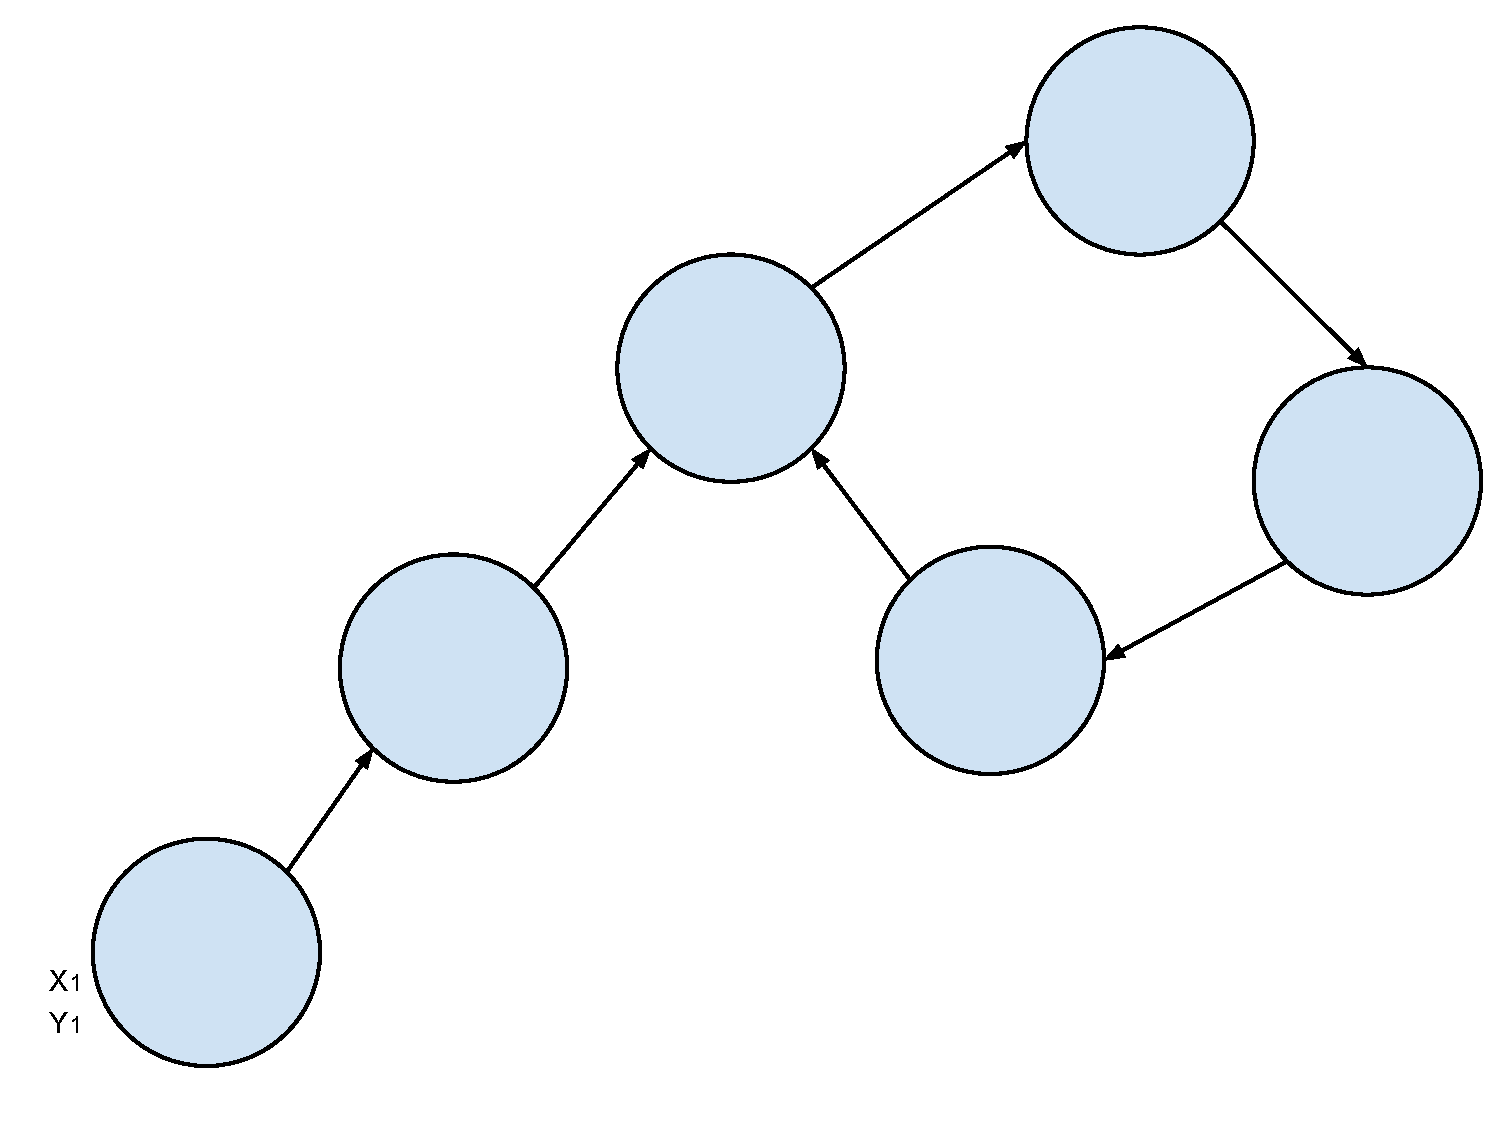
\includegraphics[width=0.7\linewidth]{Rho1}
    	\caption{Schritt 1}
    	\label{fig:Rho1)}
    \end{figure}
    
    Der Hase, hier dargestellt durch Y und der Igel, hier dargestellt durch X starten an der gleichen Position. Der Igel bewegt sich um ein Element, der Hase um zwei Elemente fort.

  \begin{figure}[!h] 
  	\centering
  	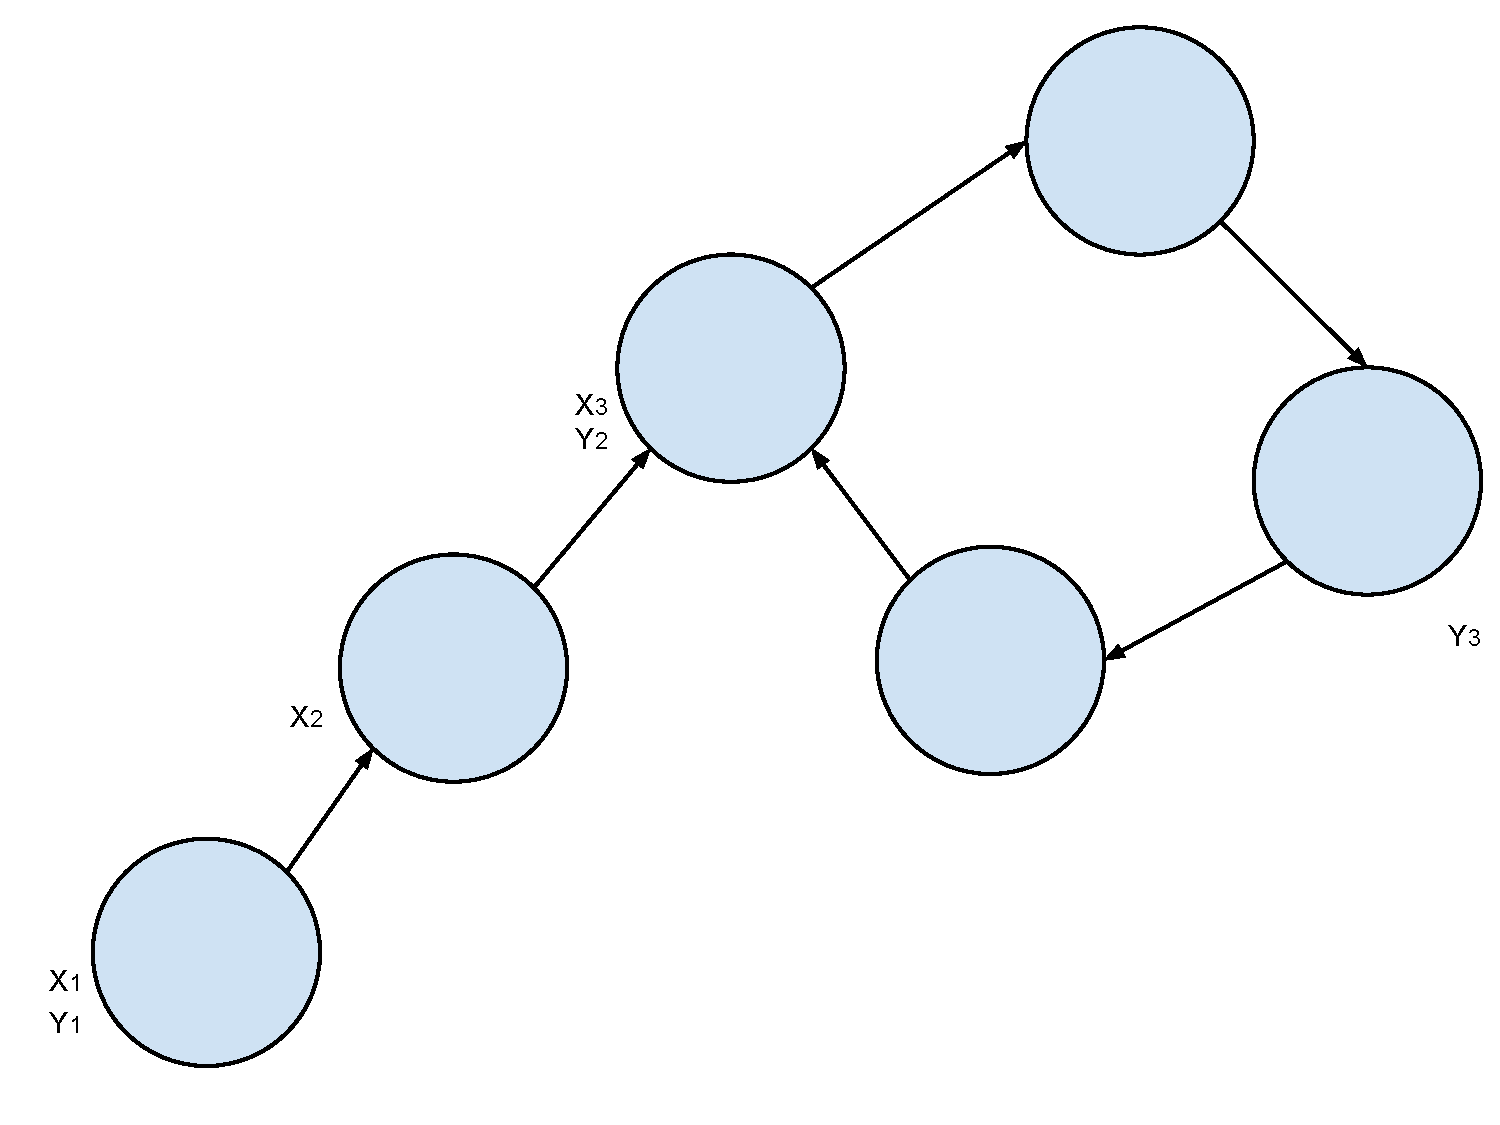
\includegraphics[width=0.7\linewidth]{Rho2}
  	\caption{Schritt 2}
  	\label{fig:Rho2)}
  \end{figure}
  
  Das ist der Zustand, bevor der Hase das erste mal im Kreis l\"auft. Es ist zu erkennen, dass der Hase doppelt so weit ist, wie der Igel.
  
    \begin{figure}[!h] 
    	\centering
    	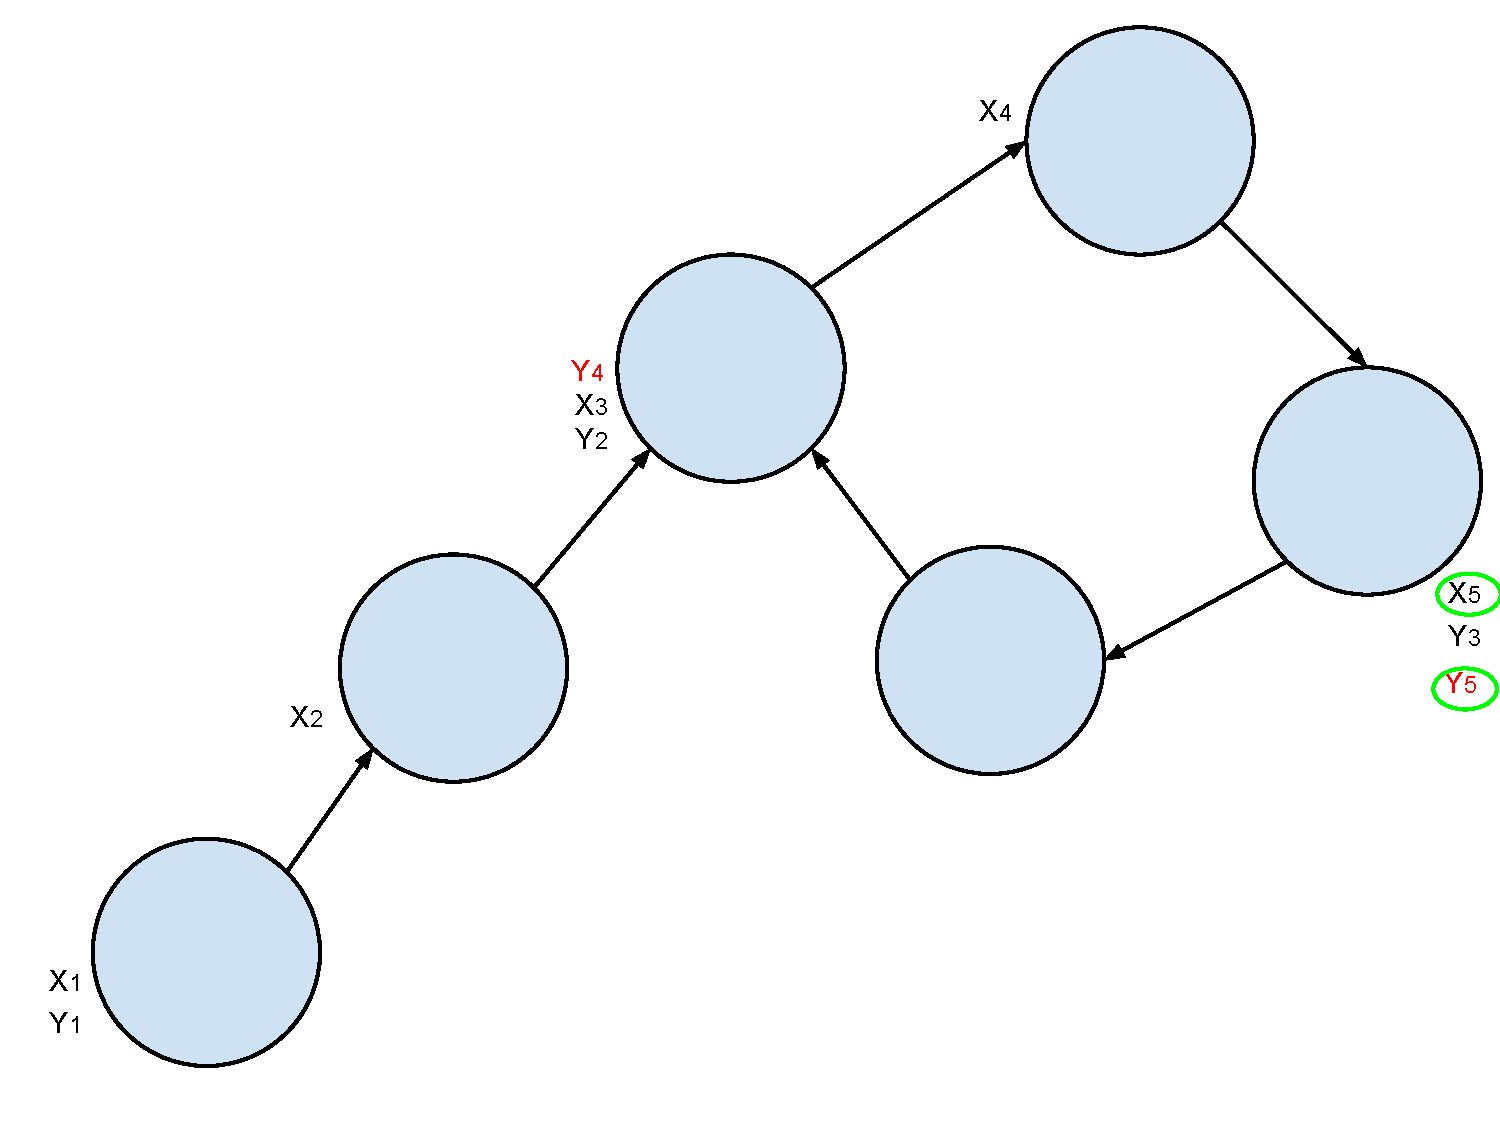
\includegraphics[width=0.7\linewidth]{Rho3}
    	\caption{Schritt 3}
    	\label{fig:Rho3)}
    \end{figure}
    Dies ist der Zustand, wenn Hase und Igel sich treffen. Die roten Zahlen zeigen, dass der Hase im Kreis l\"auft und die gr\"un eingekreisten Zahlen zeigen, dass Hase und Igel sich in ihrem f\"unften Schritt treffen. 

  \subsubsection{Mathematik}
  \begin{itemize}


  	\item Sei $M$ eine endliche Menge mit der Abbildung $f : M \rightarrow M$. Die Menge $M$ wird im Beispiel durch die Kreise dargestellt, die Abbildung $f$ durch die Pfeile, die die Kreise verbinden.
  	
  	\item Man w\"ahle $x_0 \in M$ und erzeuge die Folge $x_0, x_1, x_2,...$ mit $x_{i+1} = f(x_i)$. Dies wird im Beispiel durch den Igel dargestellt, der sich entlang der Pfeile mit einer Schrittweite von $1$ durch die Menge bewegt.
	
  	\item $\exists \ i,j \in \mathbb{N}$, sodass $i \not= j$ und $x_i = x_j$ gilt. Hiermit wird gesagt, dass es einen Zyklus gibt. Wenn der Igel zwei mal auf das gleiche Feld kommt, muss er im Kreis gegangen sein.
  	
  	\item Die Folge $y_0, y_1, y_2,...$ gegeben durch $y_0=x_0$ und $y_{i+1}=f(f(y_i))$ ist gleich der Folge $x_0,x_2,x_4,...$.\\
  Hiermit wird der Hase beschrieben, der sich doppelt so schnell bewegt wie der Igel. 
  	
  	\item Es gibt ein $c>0$, sodass $x_c=x_{2c}$.\\
  	Dies ist die Bedingung daf\"ur, dass es m\"oglich ist, dass sich Hase und Igel wieder treffen und zwar wenn beide gleich viele Schritte gemacht haben. $c$ f\"ur den Igel, $2c$ f\"ur den Hasen, da der Hase eine doppelt so gro\ss e Schrittweite hat wie der Igel.
  \end{itemize}
  
  Ein Beweis f\"ur diesen Algorithmus wird in Abschnitt \ref{sec:pollardBeweis} gef\"uhrt.
 	\subsection{Pollard Rho Algorithmus}
 	\subsubsection{Kongruenz modulo p}
 %	a  b (mod p) , p|(a − b)
 	I a = p · x + r, b = p · y + r
 	I a − b = p(x − y) + (r − r) = p(x − y)
 	I p|p(x − y)
 	7
 	\subsubsection{Idee}
 	\subsubsection{Beispiel}
 	\subsubsection{Mathematik}
 	\label{sec:pollardBeweis}
 	\subsection{Komplexit\"at}		
	\newpage
	%this file is prim_conclusion.tex

	\section{Fazit}
	\label{conclusion}
	
	
	\newpage
	\begin{thebibliography}{2}
		\bibitem[Lauritzen]{lau} \emph{Niels Lauritzen. Concrete Abstract Algebra. Reptrinted with
			corrections 2006}
		\bibitem[bk2boint]{bk2} \emph{blub}
	\end{thebibliography}
	
\end{document}